% OWD 2024
%
\documentclass{beamer}
\usepackage{subcaption}

\usetheme{CambridgeUS}
\numberwithin{figure}{section}
\beamerdefaultoverlayspecification{< +->}

\newcommand\shortauthor{ENG1 Group 23 (Cohort 3)}
\newcommand\userurl[1]{\begingroup\color{blue}\url{#1}\endgroup}
\newcommand\demomark[1]{%
    \pause[\thebeamerpauses]\vfill\centering%
    \emph{\color{gray}Live demonstration: #1}%
}

\title[Assessment 1 Presentation]{\emph{Heslington Hustle} Assessment 1
    Presentation}
\subtitle{\shortauthor}

\author[\shortauthor]{%
    \texorpdfstring{%
        \renewcommand\arraystretch{1.5}
        \begin{tabular}{ccc}
            Oliver Dixon & George Cranton & Praj Dethekar \\
            Denys Sova & Shivan Ramharry & Albara Shoukri \\
            & Rafael Duarte &
        \end{tabular}
    }{\shortauthor}
}

\institute[]{Department of Computer Science, University of York}
\date{Semester 2, 2024}

\begin{document}
\frame{\titlepage}
\begin{frame}
    \frametitle{Extensible Architecture}
    \begin{itemize}
        \item The software architecture has been designed specifically for the Assessment 2 requirements.
        \item \emph{Functionally minimal; architecturally maximal.}
        \item Case-in-point: the MVC architecture employed for the management of player and world metrics.
            Adding metrics and modifying their behaviour and visualisation schema requires minimal changes to the
            constructors.
    \end{itemize}

    \demomark{Adding an energy metric (as per Assessment 2)}
\end{frame}
\begin{frame}
    \frametitle{Simple and Modular Area Definitions}
    \begin{itemize}
        \item Areas are composed of a tilemap background, the player-controlled character, and various interactable
            objects.
        \item As such, adding, removing, or modifying on-screen entities is trivial and supported by an
            \texttt{AreaFactory}.
        \item Interactable actions are described by lambda functions, hence any interactable object can execute
            arbitrary code upon player interaction.
    \end{itemize}

    \demomark{Adding an interactable}
\end{frame}
\begin{frame}
    \frametitle{Comprehensive and Consistent Documentation}
    \begin{itemize}
        \item Every package, class, interface, method, attribute, and constant has been annotated with consistent and
            accurate JavaDoc documentation.
        \item This can be accessed during development with any IDE, or browsed interactively on-line:
            \userurl{https://www-users.york.ac.uk/~od641/ENG1-website/javadoc/index.html}
            \par\vfill%
            \begin{center}
                \fbox{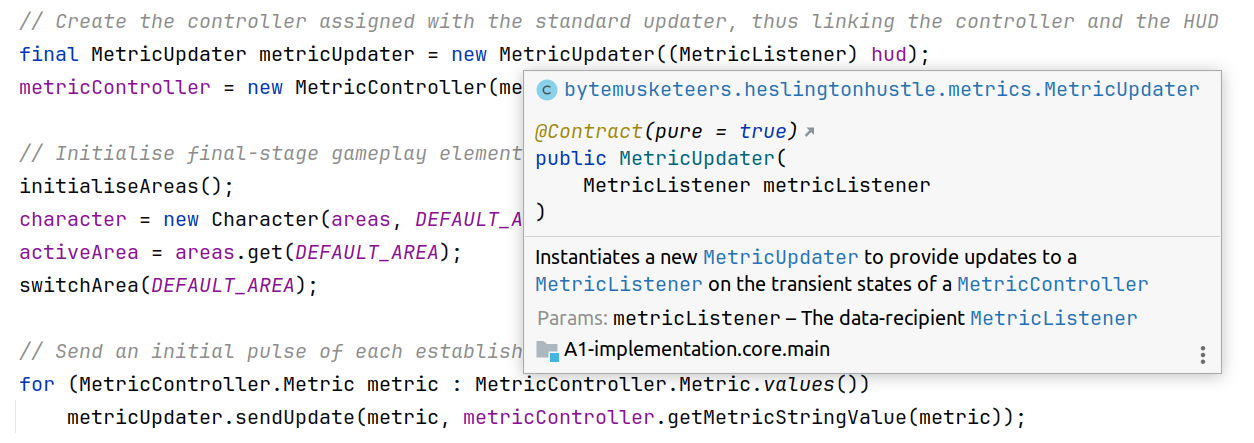
\includegraphics[width=.65\textwidth]{javadoc-ide}}
            \end{center}
    \end{itemize}
\end{frame}
\begin{frame}
    \frametitle{Any Questions?}

    \begin{center}
        
\includegraphics[width=.5\textwidth]{logo}
        \vfill
        \parbox{\textwidth}{%
            \centering\addtolength\parskip{1ex}%
            \shortauthor\par%
            \userurl{https://www-users.york.ac.uk/~od641/ENG1-website}%
        }
    \end{center}
\end{frame}
\end{document}
